%%%%%%%%%%%%%%%%%%%%%%%%%%%%%%%%%%%%%%%%%%%%%%%%%%%%%%%%%%%%%%%%%%%%%%%%%%%%%%%
% Uni Duesseldorf
% Lehrstuhl fuer Datenbanken und Informationssysteme
% Vorlage fuer Bachelor-/Masterarbeiten
% Optimiert fuer den Original-Latex-Kompiler LATEX.EXE (LaTeX=>PS=>PDF)
% Version 1.4 - 2.3.2010
%%%%%%%%%%%%%%%%%%%%%%%%%%%%%%%%%%%%%%%%%%%%%%%%%%%%%%%%%%%%%%%%%%%%%%%%%%%%%%%

%%%%%%%%%%%%%%%%%%%%%%%%%%%%%%%%%%%%%%%%%%%%%%%%%%%%%%%%%%%%%%%%%%%%%%%%%%%%%%%
%%%%%%%%%%% BEGINN EINSTELLUNG FUER DIE ARBEIT. UNBEDINGT ERFORDERLICH! %%%%%%%
%%%%%%%%%%%%%%%%%%%%%%%%%%%%%%%%%%%%%%%%%%%%%%%%%%%%%%%%%%%%%%%%%%%%%%%%%%%%%%%
% Geben Sie Ihren Namen hier an
\newcommand{\bearbeiter}{Alina Elterman}

% Geben Sie hier den Titel Ihrer Arbeit an
\newcommand{\titel}{Game-theoretic Analysis of Strategyproofness in Cake-cutting Protocols}

% Geben Sie das Datum des Beginns und Ende der Bachelorarbeit ein
\newcommand{\beginndatum}{01. September 2011}
\newcommand{\abgabedatum}{05.~Dezember~2011}

% Geben Sie die Namen des Erst- und Zweitgutachters an
\newcommand{\erstgutachter}{Prof. Dr.~J\"org Rothe}
\newcommand{\zweitgutachter}{Prof. Dr.~Peter Kern}

% Falls Sie die Arbeit zweiseitig ausdrucken wollen,
% benutzen Sie die folgende Zeile mit
% \AN fuer zweiseitigen Druck
% \AUS fuer einseitigen Druck
\newcommand{\zweiseitig}{\AUS}

% Falls die Arbeit in englischer Sprache verfasst 
% werden soll, dann benutzen Sie die folgende Zeile mit
% englisch fuer englische Sprache
% deutsch fuer deutsche Sprache
\newcommand{\sprache}{englisch}
%%%%%%%%%%%%%%%%%%%%%%%%%%%%%%%%%%%%%%%%%%%%%%%%%%%%%%%%%%%%%%%%%%%%%%%%%%%%%%%%%
%%%%%%%%%%%%%%%%%%%%%%%%%%%%%%% ENDE EINSTELLUNGEN %%%%%%%%%%%%%%%%%%%%%%%%%%%%%%
%%%%%%%%%%%%%%%%%%%%%%%%%%%%%%%%%%%%%%%%%%%%%%%%%%%%%%%%%%%%%%%%%%%%%%%%%%%%%%%%%

% Die folgende Zeile NICHT EDITIEREN oder loeschen
% (Zum Ab�ndern der BA-Vorlage in eine MA-Vorlage muessen sie
% jedoch die Datei titelmakros1.tex selbst editieren.)
%%%%%%%%%%%%%%%%%%%%%%%%%%%%%%%%%%%%%%%%%%%%%%%%%%%%%%%%%%%
% Obere Titelmakros. Editieren Sie diese Datei nur, wenn
% Sie sich ABSOLUT sicher sind, was Sie da tun!!!
% (Z.B. zum Abaendern der BA-Vorlage in eine MA-Vorlage)
% Uni Duesseldorf
% Lehrstuhl fuer Datenbanken und Informationssysteme
% Version 2.2 - 2.3.2010
%%%%%%%%%%%%%%%%%%%%%%%%%%%%%%%%%%%%%%%%%%%%%%%%%%%%%%%%%%%
\newcommand{\AN}{twoside}
\newcommand{\AUS}{}
%\newcommand{\englisch}{}
%\newcommand{\deutsch}{\usepackage[german]{babel}}

%% Die folgenden auskommentierten Optionen dienen der automatischen
%% Erkennung des Latex-Kompilers und dem Setzen der davon abh�ngigen
%% Einstellungen. Bei Problem z.B. mit dem Einbinden von verschiedenen
%% Grafiktypen bei Verwendung von PdfLatex oder Latex, einfach die
%% verschiedenen \usepackage(s) ausprobieren. (Mit diesen Einstellungen
%% funktionierte diese Vorlage bei der Verwenundg von latex.exe als
%% Kompiler bei den meisten Studierenden.)

%\newif\ifpdf \ifx\pdfoutput\undefined
%\pdffalse % we are not running pdflatex
%\else
%\pdfoutput=1 % we are running pdflatex
%\pdfcompresslevel=9 % compression level for text and image;
%\pdftrue \fi

\documentclass[11pt,a4paper, \zweiseitig]{article}



%\usepackage[iso]{umlaute}
\usepackage[latin1]{inputenc}
\usepackage{palatino} % palatino Schriftart
%\usepackage{makeidx} % um ein Index zu erstellen
\usepackage{tocbibind}
\usepackage[T1]{fontenc} %fuer richtige Trennung bei Umlauten
\usepackage{fancybox} % fuer die Rahmen
\usepackage{shortvrb}
\usepackage{ifthen}
\ifthenelse{\equal{\sprache}{deutsch}}{\usepackage[ngerman]{babel}}{}

\usepackage{lmodern} 
\usepackage{amsmath}
\usepackage{amssymb}
\usepackage{pdfpages}
\usepackage{hyperref}
%\usepackage{fancyheadings}
\usepackage{fancyhdr}
\usepackage{amsfonts}
\usepackage{amsthm}
\usepackage{color}
\usepackage{stmaryrd}
\usepackage{nomencl}
\usepackage[normalem]{ulem} 
\newcommand{\markup}[1]{\uline{#1}}
% Befehl umbenennen in abk
\let\abk\nomenclature

\usepackage{a4wide} % ganze A4 Weite verwenden

%\ifpdf
%\usepackage[pdftex,xdvi]{graphicx}
%\usepackage{thumbpdf} %thumbs fuer Pdf
%\usepackage[pdfstartview=FitV]{hyperref} %anklickbares Inhaltsverzeichnis
%\else
\usepackage[dvips,xdvi]{graphicx}
\usepackage{hyperref} %anklickbares Inhaltsverzeichnis
%\fi

%%%%%%%%%%%%%%%%%%%%%%% Massangaben fuer die Arbeit %%%%%%%%%%%%%%%
\setlength{\textwidth}{15cm}

\setlength{\oddsidemargin}{35mm}
\setlength{\evensidemargin}{25mm}

\addtolength{\oddsidemargin}{-1in}
\addtolength{\evensidemargin}{-1in}

%\makeindex
% Umgebungen f"ur S�tze usw.
\newtheorem*{bemerkung*}{Bemerkung}
\newtheorem*{defi}{Definition}
\newtheorem*{defi*}{Definition}
\newtheorem*{bezeichnungen}{Bezeichnungen}
\newtheorem*{fakt}{Fakt}
\newtheorem*{beispiel}{Beispiel}
\newtheorem*{bsp}{Beispiel}
\newtheorem*{beispiel*}{Beispiel}
\newtheorem*{satz}{Satz}
\newtheorem*{satz*}{Satz}
\newtheorem*{lem}{Lemma}
\newtheorem*{protokoll*}{Protokoll}
\newtheorem*{idee}{Idee}

%definition of new commands
\newcommand{\DGEF}{\text{\textbf{DGEF}}}

\begin{document}

%\setcounter{secnumdepth}{4} %Nummerieren bis in die 4. Ebene
%\setcounter{tocdepth}{4} %Inhaltsverzeichnis bis zur 4. Ebene

\pagestyle{headings}

\sloppy % LaTeX ist dann nicht so streng mit der Silbentrennung
\MakeShortVerb{\�}

\parindent0mm
\parskip0.5em


{
\textwidth170mm 
\oddsidemargin30mm 
\evensidemargin30mm 
\addtolength{\oddsidemargin}{-1in}
\addtolength{\evensidemargin}{-1in}

\parskip0pt plus2pt

% Die Raender muessen eventuell fuer jeden Drucker individuell eingestellt
% werden. Dazu sind die Werte fuer die Abstaende `\oben' und `\links' zu
% aendern, die von mir auf jeweils 0mm eingestellt wurden.

%\newlength{\links} \setlength{\links}{10mm}  % hier abzuaendern
%\addtolength{\oddsidemargin}{\links}
%\addtolength{\evensidemargin}{\links}

\begin{titlepage}
\vspace*{-1.5cm}
  \raisebox{17mm}{
    \begin{minipage}[t]{70mm}
      \begin{center}
        %\selectlanguage{german}
        {\Large INSTITUT F�R INFORMATIK\\}
        {\normalsize
          Lehrstuhl f�r Komplexit\"atstheorie und Kryptologie
\\
        }
        \vspace{3mm}
        {\small Universit�tsstr. 1 \hspace{5ex} D--40225 D�sseldorf\\}
     \end{center}
    \end{minipage}
  }
  \hfill
  
\includegraphics[width=130pt]{bilder/HHU_Logo}
  \vspace{14em}

% Titel
  \begin{center}
      	\baselineskip=55pt
    	\textbf{\huge \titel}
  	 	\baselineskip=0 pt
   \end{center}

  %\vspace{7em}

\vfill

% Autor
  \begin{center}
    \textbf{\Large
      \bearbeiter
    }
  \end{center}

  \vspace{35mm}
 
% Pr�fungsordnungs-Angaben
  \begin{center}
    %\selectlanguage{german}
    
%%%%%%%%%%%%%%%%%%%%%%%%%%%%%%%%%%%%%%%%%%%%%%%%%%%%%%%%%%%%%%%%%%%%%%%%%
% Ja, richtig, hier kann die BA-Vorlage zur MA-Vorlage gemacht werden...
%%%%%%%%%%%%%%%%%%%%%%%%%%%%%%%%%%%%%%%%%%%%%%%%%%%%%%%%%%%%%%%%%%%%%%%%%
    {\Large Bachelorarbeit}

    \vspace{2em}

    \begin{tabular}[t]{ll}
      Beginn der Arbeit:& \beginndatum \\
      Abgabe der Arbeit:& \abgabedatum \\
      Gutachter:         & \erstgutachter \\
                         & \zweitgutachter \\
    \end{tabular}
  \end{center}

\end{titlepage}

}

%%%%%%%%%%%%%%%%%%%%%%%%%%%%%%%%%%%%%%%%%%%%%%%%%%%%%%%%%%%%%%%%%%%%%
\clearpage
\begin{titlepage}
  ~                % eine leere Seite hinter dem Deckblatt
\end{titlepage}
%%%%%%%%%%%%%%%%%%%%%%%%%%%%%%%%%%%%%%%%%%%%%%%%%%%%%%%%%%%%%%%%%%%%%
\clearpage
\begin{titlepage}
\vspace*{\fill}

\section*{Erkl�rung}

%%%%%%%%%%%%%%%%%%%%%%%%%%%%%%%%%%%%%%%%%%%%%%%%%%%%%%%%%%%
% Und hier ebenfalls ggf. BA durch MA ersetzen...
%%%%%%%%%%%%%%%%%%%%%%%%%%%%%%%%%%%%%%%%%%%%%%%%%%%%%%%%%%%

Hiermit versichere ich, dass ich diese Bachelorarbeit
selbstst�ndig verfasst habe. Ich habe dazu keine anderen als die
angegebenen Quellen und Hilfsmittel verwendet.

\vspace{25 mm}

\begin{tabular}{lc}
D�sseldorf, den \abgabedatum \hspace*{2cm} & \underline{\hspace{6cm}}\\
& \bearbeiter
\end{tabular}

\vspace*{\fill}
\end{titlepage}

%%%%%%%%%%%%%%%%%%%%%%%%%%%%%%%%%%%%%%%%%%%%%%%%%%%%%%%%%%%%%%%%%%%%%
% Leerseite bei zweiseitigem Druck
%%%%%%%%%%%%%%%%%%%%%%%%%%%%%%%%%%%%%%%%%%%%%%%%%%%%%%%%%%%%%%%%%%%%%

\ifthenelse{\equal{\zweiseitig}{twoside}}{\clearpage\begin{titlepage}
~\end{titlepage}}{}

%%%%%%%%%%%%%%%%%%%%%%%%%%%%%%%%%%%%%%%%%%%%%%%%%%%%%%%%%%%%%%%%%%%%%
\clearpage
\begin{titlepage}

\section*{\ifthenelse{\equal{\sprache}{deutsch}}{Zusammenfassung}{Abstract}}


%%%%%%%%%%%%%%%%%%%%%%%%%%%%%%%%%%%%%%%%%%%%%%%%%%%%%%%%%%%%%%%%%%%%%%%%%%%%%%%%%
%%%%%%%%%%%%%%%%%%%%%%%%%%%% BEGINN ZUSAMMENFASSUNG %%%%%%%%%%%%%%%%%%%%%%%%%%%%%
%%%%%%%%%%%%%%%%%%%%%%%%%%%%%%%%%%%%%%%%%%%%%%%%%%%%%%%%%%%%%%%%%%%%%%%%%%%%%%%%%
Hier kommt eine ca.\ einseitige Zusammenfassung der Arbeit rein.

%%%%%%%%%%%%%%%%%%%%%%%%%%%%%%%%%%%%%%%%%%%%%%%%%%%%%%%%%%%%%%%%%%%%%%%%%%%%%%%%%
%%%%%%%%%%%%%%%%%%%%%%%%%%%%% ENDE ZUSAMMENFASSUNG %%%%%%%%%%%%%%%%%%%%%%%%%%%%%%
%%%%%%%%%%%%%%%%%%%%%%%%%%%%%%%%%%%%%%%%%%%%%%%%%%%%%%%%%%%%%%%%%%%%%%%%%%%%%%%%%

% Die folgende Zeile NICHT EDITIEREN oder loeschen
%%%%%%%%%%%%%%%%%%%%%%%%%%%%%%%%%%%%%%%%%%%%%%%%
% Untere Titelmakros. Editieren Sie diese Datei nur, wenn Sie sich
% ABSOLUT sicher sind, was Sie da tun!!!
%%%%%%%%%%%%%%%%%%%%%%%%%%%%%%%%%%%%%%%%%%%%%%%
\vspace*{\fill}
\end{titlepage}

%%%%%%%%%%%%%%%%%%%%%%%%%%%%%%%%%%%%%%%%%%%%%%%%%%%%%%%%%%%%%%%%%%%%%
% Leerseite bei zweiseitigem Druck
%%%%%%%%%%%%%%%%%%%%%%%%%%%%%%%%%%%%%%%%%%%%%%%%%%%%%%%%%%%%%%%%%%%%%
\ifthenelse{\equal{\zweiseitig}{twoside}}
  {\clearpage\begin{titlepage}~\end{titlepage}}{}
%%%%%%%%%%%%%%%%%%%%%%%%%%%%%%%%%%%%%%%%%%%%%%%%%%%%%%%%%%%%%%%%%%%%%
\clearpage 
\tableofcontents
\thispagestyle{empty}
%\enlargethispage{\baselineskip}
\clearpage \setcounter{page}{1}
%%%%%%%%%%%%%%%%%%%%%%%%%%%%%%%%%%%%%%%%%%%%%%%%%%%%%%%%%%%%%%%%%%%%%
% Leere Seite, falls Inhaltsverzeichnis mit ungerader Seitenzahl und 
% doppelseitiger Druck
%%%%%%%%%%%%%%%%%%%%%%%%%%%%%%%%%%%%%%%%%%%%%%%%%%%%%%%%%%%%%%%%%%%%%
\ifthenelse{ \( \equal{\zweiseitig}{twoside} \and \not \isodd{\value{page}} \)}
	{\pagebreak \thispagestyle{empty} \cleardoublepage}{\clearpage}



%%%%%%%%%%%%%%%%%%%%%%%%%%%%%%%%%%%%%%%%%%%%%%%%%%%%%%%%%%%%%%%%%%%%%
%%%%%%%%%%%%%%%%%%%%%%%%% BEGINN TEXTTEIL %%%%%%%%%%%%%%%%%%%%%%%%%%%
%%%%%%%%%%%%%%%%%%%%%%%%%%%%%%%%%%%%%%%%%%%%%%%%%%%%%%%%%%%%%%%%%%%%%
\section{Inroduction}
Cake Cutting is an interdisciplinairy field which is commonly researched and part of economics, political science, mathematics, operations research, and computer science. Game Theory is fulfilling the same property. Except for the fact, they have hardly something in common. While CC is about a fair division of a heterogenous divisible good, game theory is used for mathematically defining lifes procceses and analysing them.
%\begin{itemize}
%\item{division of sports tickets, health resources, computer networking resources, voting power, intellectual property licenses, costs for environmental improvements, etc}
%\item{formalize fairness, including max-min fairness, proportional fairness, envy-free fairness, etc. which may or may not lead to stable allocations in the sense of say Nash Equilibrium, or strong Nash Equilibrium}
%\end{itemize}
\pagebreak

\section{Preliminaries}
\subsection{Preliminaries of Game Theory}
\newpage
\subsection{Preliminaries of Cake-cutting}
\subsubsection{Basics}
First of all we need to define the components of cake-cutting. The following example sketches the problem statement.\\
\begin{bsp}
It was the year 1922 in London, Alan Mathison Turing was visiting a friend on his birthday. There was aswell Vilfredo Federico Pareto, Karl Popper, Felix Hausdorff und Charles West Churchman.
\end{bsp}
Now, what exactly is cake-cutting about? It involves a discrete set of $n \in \mathbb{N}$ agents (or players\footnote{common used in the game theoretic sence} ) $P_n=\{p_1,\cdots,p_n\}$. After the assumption each of them wants to get as much as possible of the good. Only the allocation of a single, divisible and heterogenous good is included in the consideration of this work. It is common to use for the visualization a rectangular cake.
\begin{center}
bild kuchen
\end{center}
The division is performed by parallel cuts. The cake $X$ is represented by the unit interval $I=[0,1] \subseteq \mathbb{R}$. Each subinterval $I'\subseteq I$ or a union of subintervals %$\bigcup\nolimits_{\m\in\mathbb{N}}I_m$ 
with $I_m\subseteq I$ is named as a boundle (piece). All boundles are disjoint. The boundle of the cake, which the player $p_i$ receives is denoted as $X_i$. When all boundles of the cake are owned by players, this state is called an \textsc{allocation}. Each piece has a public length, which can be computed as the sum of all bourderdifferences and the private value of a player.\\

Each player $p_i\in P_n$ has a valuation function (valuation) $v_i:\{X'|X' \subseteq X\} \mapsto [0,1]$ on the cake $X$ with the following properties:\\
\begin{enumerate}
\item Non-negativity\footnote{It is common to require positivity: $v_i(C)>0$ forall $C\subseteq [0,1]$ and $C \neq \emptyset$}: $v_i(C)\geq 0$ forall $C\subseteq [0,1].$
\item Normalisation: $v_i(\emptyset)=0$ and $v_i([0,1])=1.$
\item Monotonicity: if $C' \subseteq C$ then $v_i(C') \leq v_i(C).$
\item Additivity: $v_i(C \cup C')=v_i(C)+v_i(C')$ for disjoint
$C,C'\subseteq [0,1].$
\item Divisibility: forall $C\subseteq [0,1]$ and all $\alpha \in
\mathbb{R}$, $0\leq \alpha \leq 1$, exist a $B\subseteq C$, so that
$v_i(B)=\alpha \cdot v_i(C).$
\item  $v_i$ is continuous: if $0<x<y\leq 1$ with $v_i([0,x])=\alpha$ and
$v_i([0,y])=\beta$, than for every $\gamma \in [\alpha,\beta]$ there exist a $z \in [x,y]$ so that $v_i([0,z])=\gamma.$
\item Emptyness of single points:  $v_i([x,x])=0$ forall $x\in [0,1].$
\end{enumerate}

\textbf{Different Types of Fairness}\\
\newline
The goal of the fair division of a heterogeneous, continious good is to allocate the resource in a fair manner. But what is fair? It can be seen as a efficiency criteria of an allocation, which can be normalized and gives a possibility to compare different allocations. We distinguish between the following fairness criteria. \\
\begin{defi}{\textbf{(Proportional or simple fair)}}
\newline An allocation is \underline{proportional (simple fair)}, if
$v_i(X_i) \geq 1/n$ for each player $p_i \in P_N$.
\end{defi}
\begin{defi}{\textbf{(Envy-freeness)}}
\newline An allocation is \underline{envy-free}, if $v_i(X_i) \geq
v_i(X_j)$ for each couple of players $p_i, p_j \in P_N$.
\end{defi}
The following conditions can also be used on the proportional case.\\
\begin{defi}{\textbf{(Strong Envy-freeness)}}
\newline  An allocation is \underline{strong-envy-free}, if $v_i(X_i) >
v_i(X_j)$ for each couple of players $p_i, p_j \in P_N, i \neq j$.
\end{defi}
\begin{defi}{\textbf{(Super Envy-freeness)}}
\newline An allocation is \underline{super-envy-free}, if $v_i(X_j) \leq
1/n$  for each couple of players $p_i, p_j \in P_N, i \neq j$.
\end{defi}
\begin{defi}{\textbf{(Strong Super Envy-freeness)}}
\newline An allocation is \underline{stong-super-envy-free}, if $v_i(X_j) <
1/n$  for each couple of players $p_i, p_j \in P_N, i \neq j$.
\end{defi}
Hereby is the problem, that for the stronger conditions an allocations cannot exist always, like in the case when all players have equal values on the cake.\\
\newline
\textbf{Correlation between the Fairness-Properties}\\
\newline
\begin{lem}
Forall allocations \footnote{the proof can be found in \cite{}}:
\begin{enumerate}
\item Every envy-free allocation is proportional.
\item For two players an allocation is envy-free iff it is proportional.
\end{enumerate}
\end{lem}
\begin{defi}{\textbf{(Efficiency)}}
\newline An allocation is \underline{efficient (Pareto optimal)} if no other allocation exist, where one player do better, without becomming worse for an other player.
\end{defi}
\newpage
MEHR UEBER EHRLICHKEIT UND STRATEGIESICHERHEIT (mind. eine SEITE)
\subsubsection{Strategyproofness}

\begin{defi}{\textbf{(Thruthfully)}}
An allocation is \underline{thruthful} if there are no valuations where a player will do better
by lying.
\end{defi}
Only such divions are interesting, where without explicit compelling the
players to be thruthful, they will be it, because it is their best strategy
It is common that by not following the strategy of the protocol the player get into the risk to loose the garanty for their fair share. At the end of an allocation it can be proven whether every player got his fair share. 
Each protocol 

\newpage
\textbf{Different Types of Protocols}\\
\newline
Since the protocols are going to be analysed in this work, it is very important to understand the types, structure and design of them.
\textbf{Classes of Protocols}\\
\newline
Intuitive Beschreibung:(Algorithmus)
\newline In der Mathematik, Informatik und verwandten Gebieten, ist ein
\underline{Algorithmus} eine effektive Methode zur Probleml"osung, ausgedr"uckt
durch eine endliche Folge von Anweisungen.
\begin{defi}{\textbf{(Protokoll (Cake-Cutting-Protokoll))}}
\newline Ein \underline{Protokoll (Cake-Cutting-Protokoll)} ist ein adaptiver
Algorithmus mit mehreren Spielern und folgenden Eigenschaften:
\begin{itemize}
\item{It consists of rules and strategies.\\ \underline{Rules} sind
Anweisungen, die gefordert werden ohne die Bewertungen der Spieler zu kennen.\\
\underline{Strategies} sind Empfehlungen, welchen der Spieler folgen muss um
garantiert seinen gerechten Anteil zu bekommen.
}
\item{Sofern ein Spieler sich nicht an die Strategie des Protokolls h"alt,
verliert er seinen Anspruch nach einer endlichen Anzahl von Schritten ein St"uck
des Kuchens zu bekommen, welches dem geforderten Gerechtigkeitskriterium
entspricht. Sein Vorgehen hat aber keine Auswirkungen auf die Anteile der
anderen Spieler.}
\item Jeder Spieler muss zu jeder Zeit in der Lage sein v"ollig unabh"angig von
den anderen Spielern den Kuchen zu teilen (einen Schnitt zu machen).
\item Das Protokoll besitzt keine Informationen "uber die Bewertungen der
Spieler, ausser denen die angefragt wurden in dem jeweiligen oder in den
vorherigen Schritten.
\end{itemize}
\end{defi}
\begin{defi}
Ein Cake-Cutting-Protokoll wird proportional, neidfrei, stark neidfrei etc.
genannt, falls unabh"angig von den Bewertungsfunktionen der Spieler, jede
Aufteilung entsprechend proportional, neidfrei etc., unter der Vorraussetzung,
dass alle Spieler die vom Protokoll vorgegebenen Regeln und Strategien befolgen,
ist.
\end{defi}
Eines der Ziele von Cake-Cutting ist solche Protokolle anzugeben.\footnote{Siehe
auch Definition von \cite{3}, Robertson und Webb:''Approximating ...'' und
Woeginger,Sgall:''An Aproximation Scheme...'' oder
''CC\abk{CC}{\markup{C}ake-\markup{C}utting} is not a piece of cake'' von
magdon....}
\begin{defi}{\textbf{(endlich (diskret)/kontinuierlich)}}
\newline Ein \underline{endliches (diskretes)} Protokoll liefert eine L"osung
nach einer endlichen Anzahl von Entscheidungen (Bewertungen,
Markierungen,$\ldots$), dagegen muss ein Spieler bei einem
\underline{kontinuierlichen} Protokoll unendlich viele Entscheidungen treffen.
\end{defi}
\begin{defi}{\textbf{(endlich beschr"ankt/endlich unbeschr"ankt))}}
\newline Ein \underline{endlich beschr"anktes} Protokoll hat eine obere Grenze
von Schritten, welche im ung"unstigsten Fall betrachtet wird. Die gesamte Anzahl
von Entscheidungen h"angt, wenn "uberhaupt, dann nur von der Anzahl der
beteiligten Personen ab. Ein \underline{endlich unbeschr"anktes} Protokoll hat
hingegen eine nicht im Voraus absch"atzbare Anzahl.
\end{defi}
Die am meisten gesuchten Protokolle sind endlich beschr"ankt, da sie am
einfachsten in der Realit"at umsetzbar sind. Aber es gibt eine Art von
kontinuierlich Protokollen, an denen ebenfalls Interesse besteht.
\begin{defi}{\textbf{(Moving-Knife-Protokoll)}}
\newline Ein Schiedsrichter, welcher unparteisch gegen"uber den Spielern ist und
unbeteiligt an der Verteilung der St"ucke, \underline{schwenkt ein Messer
kontinuierlich} von links nach rechts und macht parallele Schnitte sofern ein
Spieler ''Halt!'' ruft. Bei manchen
MKP\abk{MKP}{\markup{M}oving-\markup{K}nife-\markup{P}rotokoll} wird der
Schiedsrichter ausgelassen und nur ein Messer oder Schwert geschwungen.
\end{defi}
\pagebreak
\subsection{The Degree of Guaranteed Envy-freeness}
\begin{description}
 \item[Motivation] For $n\geq4$ ist es offen, ob es ein neidfreies, endlich beschranktes CCP gibt!
 \item[$\Rightarrow$] Abschwachen des Ideals der Neidfreiheit. 
\end{description}
\begin{defi}
 Sei eine Aufteilung des Kuchens $X=\bigcup\limits_{i=1}^n X_i$ fur die Menge $P=\{p_1,\dots,p_n\}$ der Spieler gegeben, wobei $v_i$
 das Mass von $p_i$ und $X_i$ die Portion von $p_i$ ist.
 \begin{itemize}
  \item Eine \underline{Neidrelation}(``envy relation'') $\Vdash$ ist eine Binarrelation auf $P(\Vdash, PxP):p_i$ beneidet 
        $p_j$ $(p_i\Vdash p_j)$, $1\leq i,j\leq n,$ $i\neq j$, falls $v_i(X_i)<v_i(X_j)$.
  \item Eine \underline{Neidfrei-Relation} (``envy-free relation'') $\nVdash$ ist eine Binarrelation auf $P:p_i$ beneidet nicht $p_j$ $(p_j
        \nVdash p_j)$ ,$1\leq i,j\leq n$ ,$i\neq j$, falls $v_i(X_i)\geq v_i(X_j)$.
 \end{itemize}
\end{defi}
\underline{Eigenschaften von $\Vdash$ und $\nVdash$:}
\begin{itemize}
 \item $\Vdash$ ist irreflexiv, denn $v_i(X_i)<v_i(X_i)$ gilt nie
 \item $\nVdash$ ist reflexiv, denn $v_i(X_i)\geq v_i(X_i)$ gilt immer\\Die triviale Beziehung $p_i \nVdash p_i$ zahlt in der Regel nicht
       mit.
 \item $\Vdash$ und $\nVdash$ sind nicht transitiv.\\
       Gilt z.B. $p_i\Vdash p_j$ und $p_j\Vdash p_k$, so kann man daraus nichts uber $v_i(X_k)$ schliessen: $p_i\nVdash p_k$ ist moglich
\end{itemize}
$\Rightarrow$ Es gibt die folgenden Moglichkeiten:
\begin{enumerate}
 \item Zwei-Wege-Neid: $p_i\Vdash p_j$ und $p_j\Vdash p_i$\\(Tausch der Portionen macht beide glucklich.)
 \item Zwei-Wege-Neidfreiheit: $p_i\nVdash p_j$ und $p_j\nVdash p_i$\\(Alles ist gut.)
 \item Ein-Weg-Neid: $p_i\Vdash p_j$ und $p_j\nVdash p_i$\\
       Ein-Weg-Neidfreiheit: $p_j\Vdash p_i$ und $p_i\nVdash p_j$
\end{enumerate}
Fallerzwungene Neid- bzw. Neidfrei-Relationen: hangen ab von einem Fall geeigneter Masse.\\
Garantierte Neid- bzw. Neidfrei-Relationen: gelten in jeden Fall (auch im worst case), also unabhangig von den Massen der Spieler.\\
Anzahl garantierter Neidfrei-Relationen $=\min\limits_{alle Faelle}$ Anzahl der fallerzwungenen Neidfrei-Relationen.
\begin{beispiel*}
 Aufteilung $X=X_F\cup X_G\cup X_H$ des Kuchens mit\\
 \begin{tabular}{c|ccc}
  & $X_F=$\begin{tabular}{ccc}&&$\Box$\\&$\Box$&$\Box$\\$\Box$&$\Box$&$\Box$\\1&2&3\end{tabular}
  & $X_G=$\begin{tabular}{ccc}$\Box$&$\Box$&$\Box$\\7&8&9\end{tabular}
  & $X_H=$\begin{tabular}{ccc}$\Box$&$\Box$&$\Box$\\$\Box$&$\Box$&$\Box$\\4&5&6\end{tabular}\\ \hline \\
  F & \textcolor{blue}{$\frac{6}{18}=\frac{1}{3}$} & $\frac{6}{18}=\frac{1}{3}$ & $\frac{6}{18}=\frac{1}{3}$\\ \\
  G & $\frac{9}{18}=\frac{1}{2}$ & \textcolor{blue}{$\frac{3}{18}=\frac{1}{6}$} & $\frac{6}{18}=\frac{1}{3}$\\ \\
  H & $\frac{5}{18}$ & $\frac{7}{18}$ & \textcolor{blue}{$\frac{6}{18}=\frac{1}{3}$}
 \end{tabular}\\
 $\Rightarrow$ nicht proportional wegen $v_G(X_g)=\frac{1}{6}<\frac{1}{3}$.\\
 Es gibt:
 \begin{itemize}
  \item[] Ein-Weg-Neid von $G$ zu $F$:\\$G\Vdash F$ wegen $v_G(X_G)=\frac{1}{6}<v_G(X_F)=\frac{1}{2}$
          \\ Gleichzeitig ist dies\\$F\nVdash G$ wegen $v_F(X_G)=\frac{1}{3}=v_F(X_F)$
  \item[] Ein-Weg-Neidfreiheit von $F$ zu $G$
  \item[] Zwei-Wege-Neidfreiheit zwischen $F$ und $H$\\ $F\nVdash H$, da $v_F(X_F)=\frac{1}{3}=v_F(X_H)$\\
          $H\nVdash F$, da $v_H(X_H=\frac{6}{18}>\frac{5}{18}=v_H(X_F)$
  \item[] Zwei-Wege-Neid zwischen $G$ und $H$\\$G\Vdash H$, da $v_g(X_G)=\frac{1}{6}<\frac{1}{3}=v_G(X_H)$\\
          $H\Vdash G$, da $v_H(X_H)=\frac{1}{3}<\frac{7}{18}=v_H(X_G)$
 \end{itemize}
 %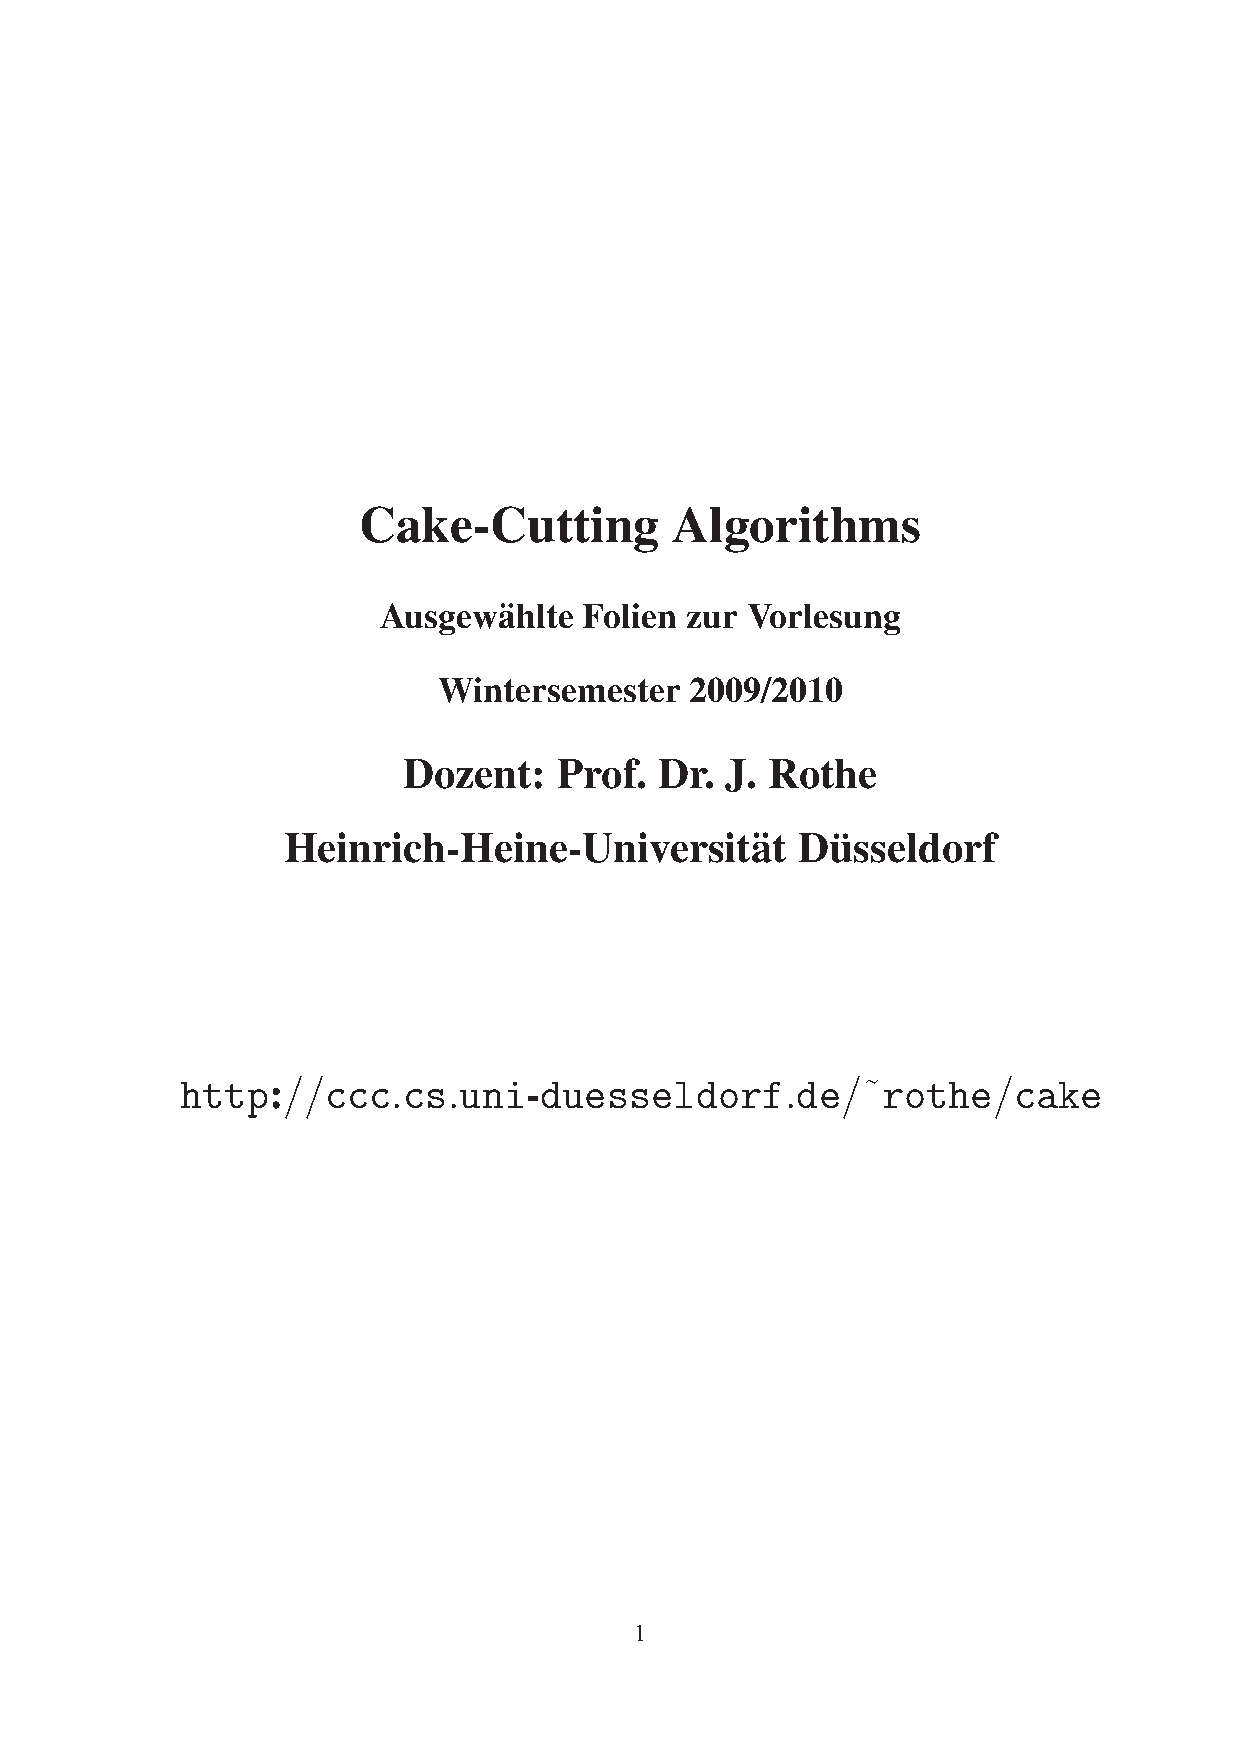
\includepdf[pages=KästchenfolieBis9,scale=0.8]{folien.pdf}
\end{beispiel*}
$\DGEF =$ Anzahl der Neidfrei-Relationen im worst case
\begin{protokoll*}
 Jorg erhalt den Kuchen.\\
 $\DGEF: n-1+(n-1)(n-2)=n-1-n^2-3n+2=n^2-2n-1$
\end{protokoll*}
\begin{satz*}
 \begin{enumerate}
  \item Jedes neidfreie CCP für $n\geq1$ Spieler hat einen $\DGEF$ von $n(n-1)$.
  \item Sei $d(n)$ der $\DGEF$ eines proportionalen CCPs mit $n\geq2$ Spielern. Dann gilt: $n\leq d(n)\leq n(n-1)$.
 \end{enumerate}
\end{satz*}
\begin{proof}
 \begin{enumerate}
  \item Da wir $p_i\nVdash p_i$ fur alle $i$, $1\leq i\leq n$, ausser 8 lassen, hat jeder der $n$ Spieler zu jedem anderen Spieler eine
        Neidfreie-Relation, insgesamt also $n(n-1)$.
  \item \begin{description}
         \item[$n=2$] Offenbar gilt: $d(2)=2$, denn da das CCP proportional ist, gilt: $v_1(X_1)\geq\frac{1}{2}$ und $v_2(X_2)\geq\frac{1}{2}
                    \Rightarrow v_1(X_1)\geq v_1(X_2)$ und $v_2(X_2)\geq v_2(X_1)$
         \item[$n\geq3$] Da $p_i\nVdash p_i$ für alle $i$ ignoriert wird, gilt $d(n)\leq n(n-1)$.
                         \begin{itemize}
                          \item[] In einer proportionalen Aufteilung gilt:\\$v_i(X_i)\geq\frac{1}{n}$ für $1\leq i\leq n$.\\
                          \item[$\Rightarrow$] Keiner der $n$ Spieler kann gleichzeitig alle anderen Spieler bendeidenl, denn:\\
                                               Angenommen, das ware nicht so. Konkret: $p_1\nVdash p_2$
                          \item[$\Rightarrow$]$v_1(X_2)>v_1(X_1)\geq\frac{1}{n}$
                          \item[$\Rightarrow$]$v_1((X-X_1)-X_2)<\frac{n-2}{n}$
                          \item[$\Rightarrow$]$(X-X_1)-X_2$ kann nicht so in $n-2$ Portionen aufgeteilt werden, dass $v_i(X_j)\geq\frac{1}{n}$
                                              für alle $j,3\leq j\leq n$, gilt.
                          \item[$\Rightarrow$]es gibt ein $j,3\leq j\leq n$, so dass $v_i(X_j)<\frac{1}{n}$, gilt.
                          \item[$\Rightarrow$]$p_i\nVdash p_j$
                         \end{itemize}
                         Also hat jeder der $n$ Spieler mindestens eine garantierte Neidfrei-Relation zu einem anderen Spieler: $n\leq d(n)$  
        \end{description}
 \end{enumerate}
\end{proof}

\begin{defi}[lemma]
 Verlangen die Regeln/Strategien eines proportionalen CCPs für $n\geq2$ Spielern von keinem Spieler, die Portionen der anderen Spieler
 zu bewerten, dann ist der $\DGEF=n$.
\end{defi}
\begin{proof}
 \begin{description}
  \item[$n=2$] Proportionalitat $\Rightarrow$ Neidfreiheit\\best case $=$ worst case\\und wie vorher: $\DGEF=2=n$
  \item[$n\geq3$] Betrachte das folgende Szenario: Für eine gegebene Aufteilung $X=\bigcup\limits_{i=1}^nX_i$, die proportional ist, aber sonst
                  keinerlei Einschrankungen unterliegt, setzen wir die Masse der Spieler so: \\Für jedes $i, 1\leq i\leq n$, bewertet $p_i$:
                  \begin{itemize}
                   \item die eigene Portion $X_i$ mit $v_i(X_i)=\frac{1}{n}=\frac{n}{n^2}\Rightarrow$ proportional!
                   \item die Portion $X_j$ eines Spielers $p_j, j\neq i: v_i(X_j)=\frac{2}{n}<\frac{1}{n}$
                   \item jede der $n-2$ übrigen Portionen $X_k$ der Spieler $p_k, |{i,j,k}|=3, v_i=(X_k)=\frac{n+1}{n^2}>\frac{1}{n}$
                  \end{itemize}
                  Insgesamt gilt dann für jedes $i, 1\leq i\leq n$:
                  \begin{enumerate}
                   \item $v_i(X)=v_i(\bigcup\limits_{j=1}^nX_j)\stackrel{\text{Additivitat}}{=}\sum\limits_{j=1}^nv_i(X_j)=
                         \frac{1}{n^2}(n+2+(n-2)(n+1))=\frac{1}{n^2}(n+2+n^2+n-2n-2)=1$
                   \item $p_i$ hat $n-2$ Neidrelationen und nur eine Neidfrei-Relation\\$\Rightarrow$ Insgesamt gibt es $n$ garantierte 
                         Neidfrei-Relationen, eine für jeden Spieler.
                  \end{enumerate}
 \end{description}
\end{proof}
\begin{satz}
 Das Last-Diminisher-Protokoll hat einen $\DGEF$ von $\frac{n(n-1)}{2}+2$
\end{satz}
\begin{proof}
 \begin{description}
  \item[Runde 1] Sei $\bar{p}_1$ der Spieler, der die erste Portion erhalt. Jeder andere Spieler bewertet diese mit $\leq\frac{1}{n}$,
                 beneidet also $\bar{p}_1$ nicht\\$\Rightarrow n-1$ garantierte Neidfrei-Relationen
  \item[Runde $i, 1<i<n$] Analog zu Runde 1 konnen $n-i$ Neidfrei-Relationen garantiert werden. $\bar{p}_i$, der die ite Portion erhalt, wird
                          von den verbleibenden Spielern nicht beneidet.\\$\Rightarrow$ mindestens $\sum\limits_{i=1}^ni=\frac{n-1}{2}$
                          garantierte Neidfrei-Relationen
  \item[Letzte Runde] \begin{enumerate}
                       \item Cut \& Choose zwischen $\bar{p}_{n-1}$ und $\bar{p}_n$. Keiner dieser beiden beneidet den anderen.\\
                             $\Rightarrow$ eine zusatzliche garantierte Neidfrei-Relation.
                       \item Da Last-Diminisher proportional ist, gibt es eine weitere garantierte Neidfrei-Relation für $\bar{p}_1$
                      \end{enumerate}
 \end{description}
$\Rightarrow\DGEF=\frac{(n-1)n}{2}+2$ 
\end{proof}
\begin{satz}
 Das Lone-Chooser-Protokoll hat einen $\DGEF$ von $n$.
\end{satz}
\begin{proof}
 Kein Spieler bewertet die Portion irgendeines anderen Spielers.\\$\stackrel{\text{Lemma}}{\Longrightarrow}\DGEF=n$
\end{proof}


\pagebreak

\section{Proportional Procedures and their DGEF}
Each proportional procedure consist of rules and strategies. Since the rules are compulsory, the strategies of e... . In this chapter the strategies of common used procedures are shown (probably specialised, if doible(?)) and explained with examples. Then their strategyproofness is analysed. During complications the effect on the DGEF is shown. Complete procedures can be found in \cite{}.
\subsection{The Steinhaus-Kuhn lone divider procedure}
\newpage
\subsection{The Banach-Knaster last-diminisher procedure}
\textbf{satz}

Falls die Bewertungsfunktionen der Spieler nicht "ubereinstimmen, gibt es eine nicht ehrliche Strategie f"ur den ersten Spieler in jeder Runde ein St"uck mit $v_i(S_i)>1/N$ zu bekommen.
\textbf{satz}
\textbf{proof}
Im Schritt 1: Das abgeschnittene St"uck soll den Wert $1/N+$ Rest von $S_1$ haben.\\
Fallunterscheidung: Entweder Spieler $p_1$ kriegt dieses St"uck oder Spieler $p_i$ beschneidet es und somit kann Spieler $p_1$ ein solches St"uck in der darauffolgenden Runde bekommen, oder bei Cut und Choose am Ende.
\textbf{proof}
\newpage
\subsection{The Fink lone-chooser procedure}
\newpage
\subsection{The Cut-Your-Own-Piece procedure}
\newpage
\subsection{The Divide-and-Conquer procedure}
\newpage
\subsection{Erweiterte procedure}
\newpage
\subsection{Erweitertung der Erweiterten procedure}
\newpage
\section{Related Work}
\pagebreak

\section{Conclusions and Open Questions/Problems}
\pagebreak

%\begin{figure}[htb]
%\begin{center}
%  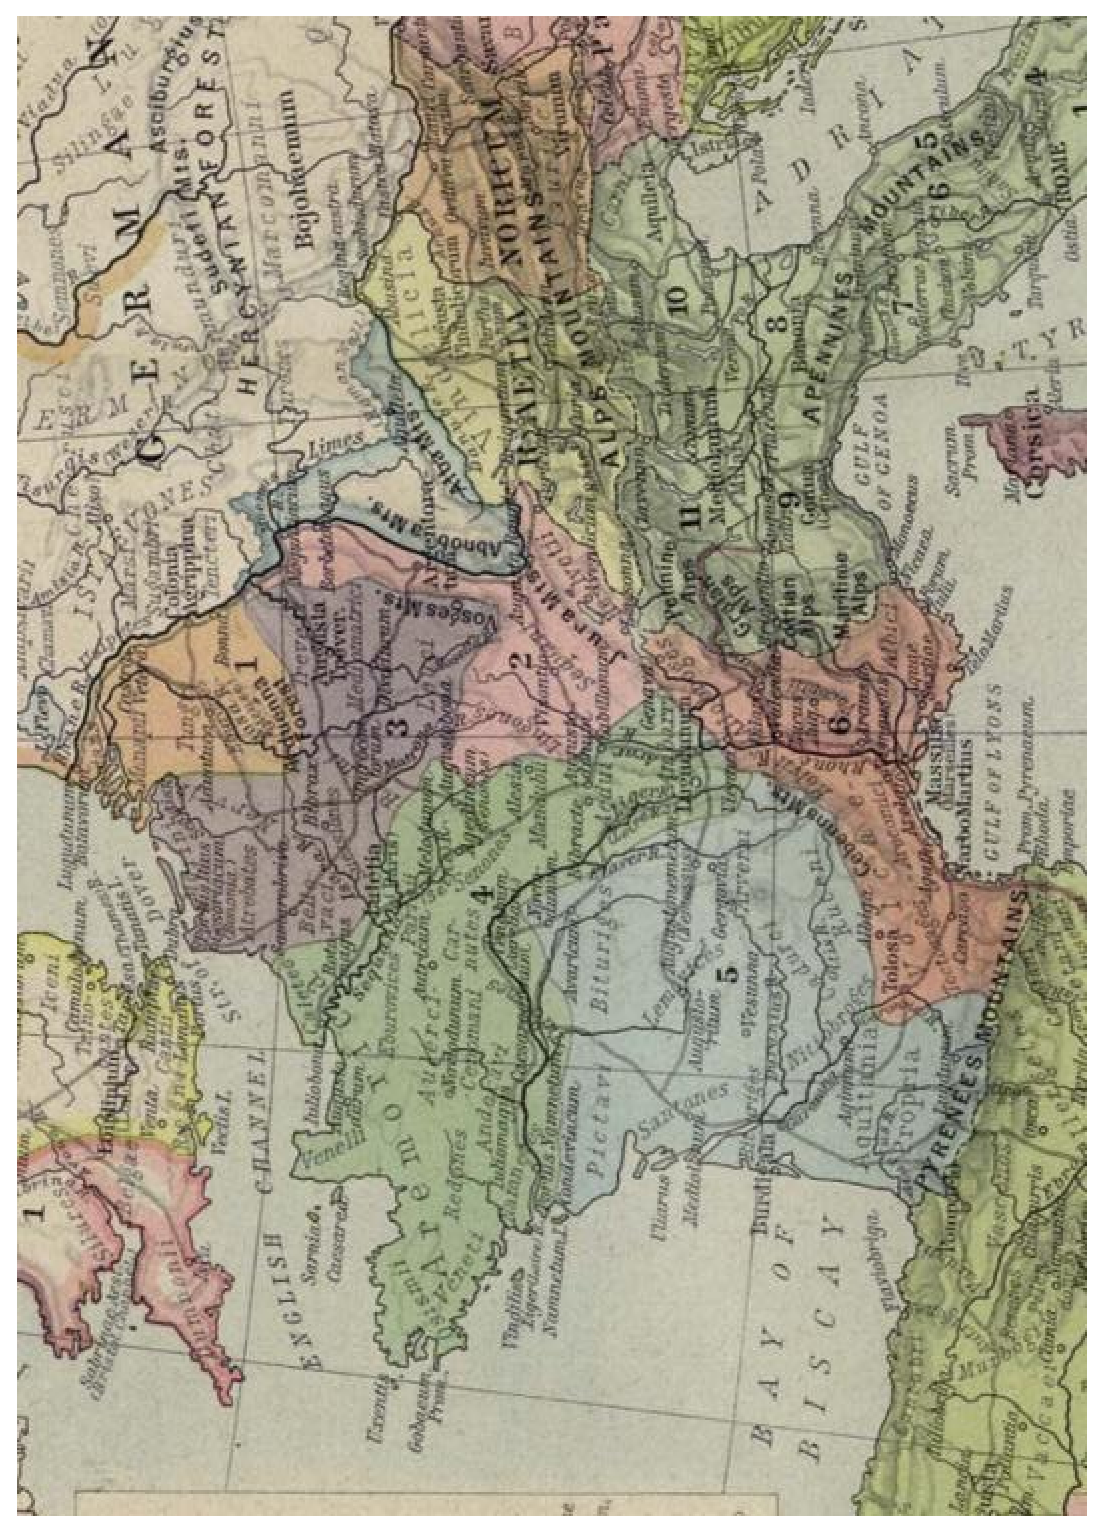
\includegraphics[width=175pt, angle=270]{bilder/Galia}
%  \caption{Gallien zur Zeit Caesars}\label{fig_Gallien}
%\end{center}
%\end{figure}


%\begin{table}[htb]
%\begin{center}
%\begin{tabular}{|l|l|l|}
%\hline
%Jahr &  Erster Consul & Zweiter Consul\\
%\hline \hline
%1 & C. Caesar         & L. Aemilius Paullus\\
%2 & P. Vinicius       & P. Alfenus Varus\\
%3 & L. Aelius Lamia   & M. Servilius\\
%4 & Sex. Aelius Catus &  C. Sentius Saturninus\\
%5 & L. Valerius Messalla& Cn. Cornelius Cinna \\
%suff. & C. Vibius Postumus &  C. Ateius Capito\\
%6 & M. Aemilius Lepidus & L. Arruntius\\
%\hline
%\end{tabular}
% \caption{R�mische Konsulen}\label{tab_Konsulen}
%\end{center}
%\end{table}


\pagebreak

%%%%%%%%%%%%%%%%%%%%%%%%%%%%%%%%%%%%%%%%%%%%%%%%%%%%%%%%%%%%%%%%%%%%%%%%%%
%%%%%%%%%%%%%%%%%%%%%%%%%%%%%%% ENDE TEXTTEIL %%%%%%%%%%%%%%%%%%%%%%%%%%%%
%%%%%%%%%%%%%%%%%%%%%%%%%%%%%%%%%%%%%%%%%%%%%%%%%%%%%%%%%%%%%%%%%%%%%%%%%%

\clearpage
\bibliography{references}
\bibliographystyle{alphadin}
%\vspace*{\fill}

\clearpage

\listoffigures

\listoftables

%\pagebreak

%\printindex
\end{document}
